% Indicate the main file. Must go at the beginning of the file.
% !TEX root = ../main.tex


%----------------------------------------------------------------------------------------
% CHAPTER 4
%----------------------------------------------------------------------------------------

\chapter{Approach}

\label{Chapter4} % For referencing the chapter elsewhere, use \ref{Chapter2} 

%----------------------------------------------------------------------------------------
In the previous chapter \ref{Chapter2} of this text, we explored four of the key pillars of \ac{DevOps}, and concluded that the related issues for solving the key problems within a \ac{SCRUM} team, and in \ac{DevOps} in general, are not a single point of truth but rather a whole web of aspects to be solved. The purpose of this chapter is to propose an approach that addresses the challenges that were identified. The focus is on the efficient management and access to information tailored to the different roles within a \ac{SCRUM} team and to improve the collaboration and productivity in the Team.


\section{Requirements and Features}

Designing successful approaches which are based on the principle that the right information needs to be available in a timely manner, tailored to the specific needs of each role within a \ac{SCRUM} team. In order to do this, the design of the approach must have the following key features as illustrated in \ref{fig:approach:1}

\begin{outline}
    \1 \textbf{Role-based Information Highlighting:}
    \2 electable roles
    \2 maintained by \ac{AI}
    \2 sorting based on keywords in text
    \2 separate pages per role
    \1 \textbf{Decision Logs Within a Mirrored Approach}
    \2 maintained
    \2 easy readable
    \2 stored in the related code base
    \2 mirrored to a centralized information storage
    \2 consistent terminology
    \1 \textbf{Infrastructure as Code}
    \2 accessible without granular access rights
    \2 contains configurations
    \2 stored at the related code base
    \2 testing on changes in the pipeline
\end{outline}

\begin{figure}[h!]
\centering
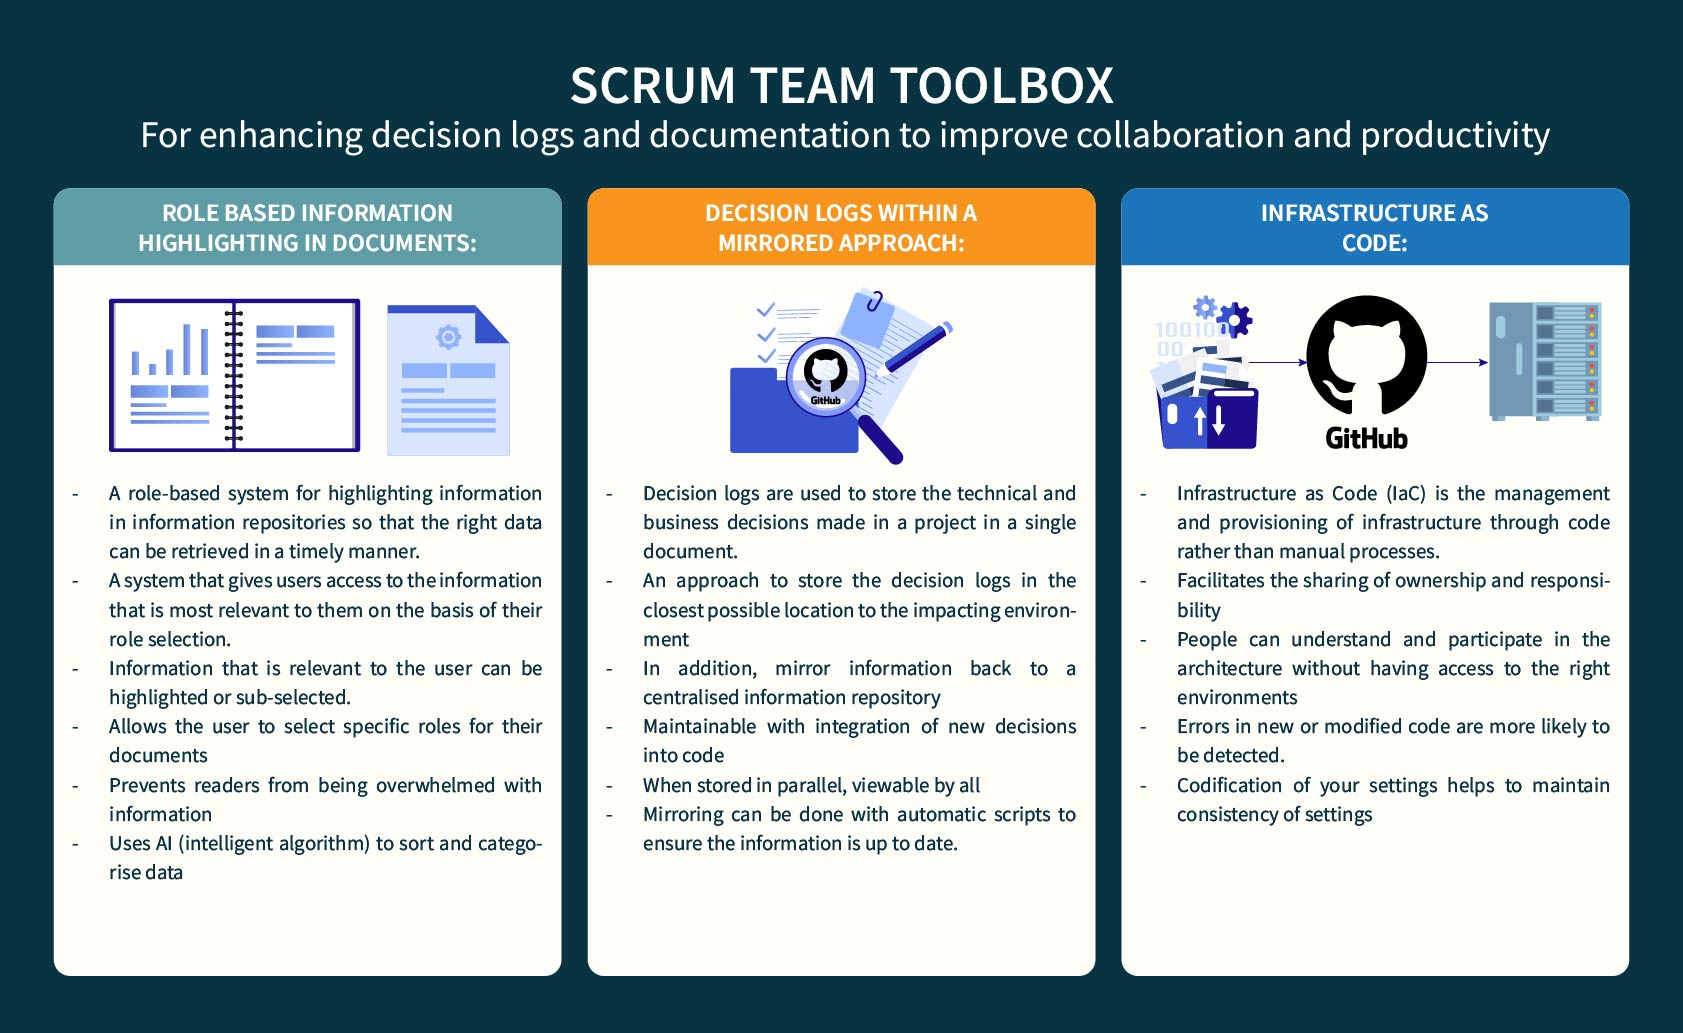
\includegraphics[width=\linewidth]{Images/toolbox.jpg}
\caption{Illustrated Features for the Approaches}
\label{fig:approach:1}
\end{figure}


\subsection*{Role-based Information Highlighting}
By selecting their role (e.g. project manager, developer), the system should allow users to access the information most relevant to their responsibilities. This will ensure that team members are not inundated with unnecessary information, thereby preventing them from becoming overwhelmed with detail and allowing them to focus on what they need to know. This process should be maintained and ensured by an \ac{AI} model, configured for the relevant roles, that attempts to highlight information based on keywords used in the text. There are also different ways of presenting this information, either on separate pages for each role or on the same page but highlighted for the appropriate role. With regard to the separation of information, there may be difficulties in extracting the correct information from the existing formats. This may be due to the fact that a significant proportion of the documentation is in the form of screenshots rather than text, and the conversion of existing documentation may present a challenge.
\subsection*{Decision Logs Within a Mirrored Approach}
The objective of decision logs is twofold. Firstly, it is to guarantee that they are consistently maintained and kept up to date. Secondly, it is to propose an approach for maintaining these data in the appropriate code base and mirroring them at the same time to a centralized document base. This is to ensure the accessibility of the information for those without direct involvement in software development. The mirroring process should be carried out by automated tools to reduce the effort required and to ensure the information's maintainability within the team. It is of the utmost importance to ensure the currency of this information in order to justify the effort invested in its maintenance. Furthermore, the formatting of the data and the use of consistent terminology and terminology that is readily comprehensible are also crucial factors.
\subsection*{Infrastructure as Code}
The integration of tooling such as Terraform\footnote{Terraform is an \ac{IaC} tool that enables you to safely and predictably provision and manage infrastructure in any cloud.} facilitates the accessibility of deployment information and configurations for the entire team. This is in contrast to the previous approach of having deployment configurations exclusive to the deployment-responsible teams. Individuals interested in gaining more information about deployments and configurations do not require special access rights to cloud infrastructure; rather, they can extract the required information from the deployment files stored in the repository. 

\section{Situation Overview}

Facing the challenge of outdated documentation and decision logs, a \ac{SCRUM} team comprising distinct personas seeks an innovative approach. This section outlines a strategy that leverages the previously defined requirements and features based on the four pillars of \ac{DevOps}: culture, automation, measurement, and knowledge sharing, to address these challenges, especially with the onboarding of two new developers: Klaus \ref{fig:persona:klaus}, a Front-End Developer, and Karin \ref{fig:persona:karin}, a Back-End Developer.

The team's current documentation and decision logs are significantly outdated. This poses a challenge for integrating Klaus \ref{fig:persona:klaus} and Karin \ref{fig:persona:karin} into the workflow efficiently. Concerns are raised by both business stakeholders and existing team members about the potential for information gaps. The team realizes the need for an updated approach to maintain their documentation and logs to ensure a smooth transition for the newcomers.

\section{Strategic Approach}
To navigate these challenges, the team decides to implement approaches which embody the core principles of \ac{DevOps}, tailored to their unique dynamics and incorporating the personas of Emma \ref{fig:persona:emma}, Lucas \ref{fig:persona:lucas}, along with Alex \ref{fig:persona:alex}, Mia \ref{fig:persona:mia}, Klaus \ref{fig:persona:klaus}, and Karin \ref{fig:persona:karin}.

\subsection*{Role-Based Information Highlighting}
As the Product Owner, Emma requires high-level overarching perspectives and clear summaries of technical decisions. The feature ensures that she is able to receive information that pertains directly to project progress without becoming overwhelmed by technical details. The role-specific information pages maintained by \ac{AI} will allow her to concentrate on strategic planning and stakeholder communication.

Lucas, the \ac{SCRUM} Master, necessitates tools for the management of workflows, performance tracking, and the resolution of impediments. The real-time updates accessible through role-based information highlighting enable the \ac{SCRUM} Master, Lucas, to address issues that may arise, thus enhancing productivity.

In terms of the specific roles of Mia and Klaus, the front-end developers, and Alex and Karin, the back-end developers, the role-based information highlighting enables them to rapidly identify detailed documentation relevant to their tasks, including \ac{UI}/\ac{UX} design principles for front-end work and \ac{API} documentation and system architecture for back-end tasks. This reduces the time spent searching for information, thus allowing the aforementioned individuals to dedicate more time to coding and problem resolution.

\subsection*{Decision Logs Within a Mirrored Approach}
It is of great importance that all team members have access to consistent, up-to-date decision logs, which should be maintained in a unified way across the entire team. Emma must be able to understand the rationale underlying technical decisions in order to effectively communicate with relevant stakeholders. Similarly, Lucas employs decision logs to track progress, thereby ensuring that all team members are aligned. For developers such as Mia, Klaus, Alex, and Karin, these logs provide contextual information and reasoning behind specific coding practices and architectural choices.

The maintenance of these logs within the relevant code base, accompanied by the mirroring of these logs to a centralised information storage, ensures that all team members have access to the same information. This process increases transparency and consistency, as well as reducing manual effort and facilitating the current and accessible maintenance of logs.

\subsection*{Infrastructure as Code}
The adoption of \ac{IaC} tools such as Terraform will facilitate the access to deployment information. This will enable Emma to gain a more comprehensive understanding of deployment processes, thereby enabling her to communicate more effectively with stakeholders regarding release schedules and deployment strategies.

For developers, such as Mia, Klaus and Alex, the implementation of \ac{IaC} tools allows for the convenient access and modification of infrastructure configurations, negating the necessity for special permissions. This facilitates a more collaborative and flexible development environment, in which changes can be tested and deployed with greater ease and confidence.

\subsection*{Implementation Steps}
\begin{outline}
    \1 \textbf{Role-Based Information Highlighting:}
        \2 develop \ac{AI} models to identify and highlight key information based on role-specific keywords.
        \2 implement into model to separate information pages for different roles.
        \2 test and refine the AI models to ensure accurate information sorting.
    \1 \textbf{Decision Logs Within a Mirrored Approach:}
        \2 set up automated script to mirror decision logs from the code base to a centralized information storage.
        \2 establish guidelines for maintaining consistent terminology and readability in decision logs.
        \2 conduct regular audits to ensure logs are up-to-date.
    \1 \textbf{Infrastructure as Code:}
        \2 train the team on \ac{IaC} tools like Terraform.
        \2 integrate \ac{IaC} practices into the development workflow.
        \2 ensure that \ac{IaC} configurations are included in the version control system and are subject to code reviews and testing.
\end{outline}

\subsection*{Expected Outcomes}
By implementing this strategic approach, the team expects to see several key benefits:
\begin{outline}
    \1 \textbf{Improved Efficiency:} team members can quickly find the information they require, improving productivity.
    \1 \textbf{Enhanced Collaboration:} transparent and accessible decision logs foster better communication and understanding among team members.
    \1 \textbf{Greater Flexibility:} the use of \ac{IaC} tools allows for easier and more flexible management of infrastructure, accommodating changes swiftly and safely.
    \1 \textbf{Seamless Onboarding:} new team members like Klaus and Karin will find it easier to integrate into the team, as they have access to up-to-date documentation and clear role-specific information.
\end{outline}

This approach ensures that each team member, from Emma and Lucas to Mia, Klaus, Alex, and Karin, can perform their roles effectively, contributing to the overall success of the \ac{SCRUM} team and the project's objectives.


\section{Conclusion}
This chapter proposes a comprehensive approach to address the challenges identified within a \ac{SCRUM} team, particularly in the context of \ac{DevOps} practices. The approach focuses on role-based information highlighting, maintaining decision logs within a mirrored approach, and integrating \ac{IaC}, with the aim of enhancing the efficiency, collaboration, and productivity of the team.

The implementation of role-based information highlighting ensures that each team member receives the specific information they require, thereby reducing the risk of information overload and enhancing focus. The maintenance of decision logs and their mirroring across the team provide consistent and accessible information, promoting transparency and understanding of technical decisions. The incorporation of \ac{IaC} tools enables the seamless access to deployment configurations, fostering a collaborative and flexible development environment.  

The implementation of these strategies addresses not only the immediate challenges faced by the team, including the integration of new team members and the need for updated documentation, but also aligns with the core principles of \ac{DevOps}: culture, automation, measurement, and knowledge sharing. This alignment ensures that the approach is robust and scalable, capable of adapting to future challenges and contributing to the continuous improvement of \ac{SCRUM} practices.

Concluding, the proposed strategic approach offers a structured solution to the multifaceted challenges of information and collaboration management in a \ac{SCRUM} team. By employing these tailored strategies, the team can achieve greater efficiency, enhanced collaboration, and improved overall productivity, ultimately leading to more successful project outcomes.




%----------------------------------------------------------------------------------------